\documentclass{article}
\usepackage[utf8]{inputenc}
\usepackage{listings}
\usepackage{multimedia} % to embed movies in the PDF file
\usepackage{graphicx}
\usepackage{comment}
\usepackage[english]{babel}
\usepackage{amsmath}
\usepackage{amsfonts}
\usepackage{subfigure}
\usepackage{wrapfig}
\usepackage{multirow}
\usepackage{tikz}
\usepackage{verbatim}

\newtheorem{theorem}{Theorem}[section]
\newtheorem{lemma}[theorem]{Lemma}
\newtheorem{corollary}[theorem]{Corollary}
%\newtheorem{algorithm}[theorem]{Algorithm}
\newtheorem{remark}[theorem]{Remark}
\newenvironment{proof}{\noindent {\bf Proof:} }{\hfill $\Box$ \\[2ex] }
\newenvironment{keywords}{\begin{quote} {\bf Key words} }
                         {\end{quote} }
\newenvironment{AMS}{\begin{quote} {\bf AMS subject classifications} }
                         {\end{quote} }


\newcommand{\eref}[1]{\mbox{\rm(\ref{#1})}}
\newcommand{\tref}[1]{\mbox{\rm\ref{#1}}}
\newcommand{\set}[2]{\left\{ #1 \; : \; #2 \right\} }
\newcommand{\deq}{\raisebox{0pt}[1ex][0pt]{$\stackrel{\scriptscriptstyle{\rm def}}{{}={}}$}}

\newcommand {\DS} {\displaystyle}

\newcommand{\real}{\mathbb{R}}
\newcommand{\compl}{\mathbb{C}}



\newcommand {\half} {\mbox{$\frac{1}{2}$}}
\newcommand{\force}{{\mathbf{f}}}
\newcommand{\strain}{{\boldsymbol{\varepsilon}}}
\newcommand{\stress}{{\boldsymbol{\sigma}}}
\renewcommand{\div}{{\boldsymbol{\nabla}}}

\newcommand {\cA} {{\cal A}}
\newcommand {\cB} {{\cal B}}
\newcommand {\cC} {{\cal C}}
\newcommand {\cD} {{\cal D}}
\newcommand {\cE} {{\cal E}}
\newcommand {\cL} {{\cal L}}
\newcommand {\cP} {{\cal P}}
\newcommand {\cQ} {{\cal Q}}
\newcommand {\cR} {{\cal R}}
\newcommand {\cV} {{\cal V}}
\newcommand {\cW} {{\cal W}}
\newcommand {\CH} {{\cal H}}
\newcommand {\CS} {{\cal S}}


\newcommand{\bzero}{\mathbf{0}}
\newcommand{\ba}{\mathbf{a}}
\newcommand{\bb}{\mathbf{b}}
\newcommand{\bc}{\mathbf{c}}
\newcommand{\bd}{\mathbf{d}}
\newcommand{\be}{\mathbf{e}}
\newcommand{\bff}{\mathbf{f}}
\newcommand{\bg}{\mathbf{g}}
\newcommand{\bh}{\mathbf{h}}
\newcommand{\bn}{\mathbf{n}}
\newcommand{\bp}{\mathbf{p}}
\newcommand{\bq}{\mathbf{q}}
\newcommand{\br}{\mathbf{r}}
\newcommand{\bs}{\mathbf{s}}
\newcommand{\bt}{\mathbf{t}}
\newcommand{\bu}{\mathbf{u}}
\newcommand{\bv}{\mathbf{v}}
\newcommand{\bw}{\mathbf{w}}
\newcommand{\bx}{\mathbf{x}}
\newcommand{\by}{\mathbf{y}}
\newcommand{\bz}{\mathbf{z}}
\newcommand{\bA}{\mathbf{A}}
\newcommand{\bB}{\mathbf{B}}
\newcommand{\bC}{\mathbf{C}}
\newcommand{\bD}{\mathbf{D}}
\newcommand{\bE}{\mathbf{E}}
\newcommand{\bF}{\mathbf{F}}
\newcommand{\bG}{\mathbf{G}}
\newcommand{\bH}{\mathbf{H}}
\newcommand{\bI}{\mathbf{I}}
\newcommand{\bJ}{\mathbf{J}}
\newcommand{\bK}{\mathbf{K}}
\newcommand{\bL}{\mathbf{L}}
\newcommand{\bM}{\mathbf{M}}
\newcommand{\bN}{\mathbf{N}}
\newcommand{\bO}{\mathbf{O}}
\newcommand{\bP}{\mathbf{P}}
\newcommand{\bQ}{\mathbf{Q}}
\newcommand{\bR}{\mathbf{R}}
\newcommand{\bS}{\mathbf{S}}
\newcommand{\bU}{\mathbf{U}}
\newcommand{\bV}{\mathbf{V}}
\newcommand{\bW}{\mathbf{W}}
\newcommand{\bX}{\mathbf{X}}
\newcommand{\bY}{\mathbf{Y}}
\newcommand{\bZ}{\mathbf{Z}}

\newcommand{\cO}{ {\cal O} }
\newcommand{\CT}{ {\cal T} }
\newcommand{\IL}{{\mathbb L}}
\newcommand{\sIL}{{{{\mathbb L}_s}}}
\newcommand{\bOmega}{{\boldsymbol{\Omega}}}
\newcommand{\bPsi}{{\boldsymbol{\Psi}}}

\newcommand{\bgamma}{{\boldsymbol{\gamma}}}
\newcommand{\bmu}{{\boldsymbol{\mu}}}
\newcommand{\blambda}{{\boldsymbol{\lambda}}}
\newcommand{\bLambda}{{\boldsymbol{\Lambda}}}
\newcommand{\bpi}{{\boldsymbol{\pi}}}
\newcommand{\bPi}{{\boldsymbol{\Pi}}}
\newcommand{\bphi}{{\boldsymbol{\phi}}}
\newcommand{\bPhi}{{\boldsymbol{\Phi}}}
\newcommand{\bpsi}{{\boldsymbol{\psi}}}
\newcommand{\btheta}{{\boldsymbol{\theta}}}
\newcommand{\bTheta}{{\boldsymbol{\Theta}}}
\newcommand{\bSigma}{{\boldsymbol{\Sigma}}}
\newcommand{\sump}{\sideset{}{^{'}}\sum} 
\DeclareMathOperator*{\Res}{Res}
\DeclareMathOperator{\OO}{O}
\DeclareMathOperator{\oo}{o}
\DeclareMathOperator{\erfc}{erfc}
\def\Xint#1{\mathchoice
   {\XXint\displaystyle\textstyle{#1}}%
   {\XXint\textstyle\scriptstyle{#1}}%
   {\XXint\scriptstyle\scriptscriptstyle{#1}}%
   {\XXint\scriptscriptstyle\scriptscriptstyle{#1}}%
   \!\int}
\def\XXint#1#2#3{{\setbox0=\hbox{$#1{#2#3}{\int}$}
     \vcenter{\hbox{$#2#3$}}\kern-.5\wd0}}
\def\ddashint{\Xint=}
\def\pvint{\Xint-}





\title{AMATH 567 Homework 3}
\author{Cade Ballew \#2120804}
\date{October 20, 2021}

\begin{document}

\maketitle

\section{Problem 1 (2.2.4)}
Consider the multi-valued function $\ln(z^\alpha)$ where $\alpha\in\mathbb{R}$. By the definition of the complex logarithm and letting $z=Re^{i\arg z}$ for any $k\in\mathbb{Z}$, 
\[
\ln(z^\alpha)=\ln(R^\alpha e^{i\alpha\arg z})=\ln(R^\alpha)+i\arg(e^{i\alpha\arg z})=\alpha\ln R+i\arg(e^{i\alpha\arg z}).
\]
Note that we have multi-valued arguments. This setup also gives that
\[
\alpha\ln z=\alpha(\ln R+i\arg z)=\alpha\ln R+\alpha i\arg z.
\]
We wish to show that the values of these two multi-valued functions are not the same. This amounts to checking whether $\arg(e^{i\alpha\arg z})=\alpha \arg z$ in general. If we let $\alpha=\frac{1}{2}$ and $z=1$ such that $\arg(z)=0$ (note that we fixed a branch to the principal argument by doing this, so $\arg(w)\in(-\pi,\pi]$ for any $w\in\mathbb{C}$), $\alpha \arg z=0$ but $\arg(e^{i\alpha(\arg z+2\pi k)})=\arg(e^{ik\pi})=\arg(\pm1)=0,\pi$ where $k\in\mathbb{C}$. Thus, the multvaluedness does not resolve here, so the sets of all values of these functions do not necessarily match. 
\section{Problem 2} 
Consider the function $w=z^z$ where $z\in\mathbb{C}$. We first find its real and imaginary parts by letting $z=Re^{i\theta}$ and writing
\[
\begin{split}
z^z&=e^{z\ln z}= e^{z(\ln R+i\theta)}=e^{R(\cos\theta+i\sin\theta)(\ln R+i\theta)}=e^{R(\cos\theta\ln R-\theta\sin\theta+i(\sin\theta\ln R+\theta\cos\theta))} \\&=
e^{R\cos\theta\ln R-R\theta\sin\theta}e^{i(R\sin\theta\ln R+R\theta\cos\theta)}\\&=
e^{R\cos\theta\ln R-R\theta\sin\theta}(\cos(R\sin\theta\ln R+R\theta\cos\theta)+i\sin(R\sin\theta\ln R+R\theta\cos\theta))
\end{split}
\]
Note that $R$ and $\theta$ are both real by definition, so we can see that 
\[
\Re(w)=e^{R\cos\theta\ln R-R\theta\sin\theta}\cos(R\sin\theta\ln R+R\theta\cos\theta)
\]
and 
\[
\Im(w)=e^{R\cos\theta\ln R-R\theta\sin\theta}\sin(R\sin\theta\ln R+R\theta\cos\theta).
\]
Let $A=R\cos\theta\ln R-R\theta\sin\theta$ and $B=R\sin\theta\ln R+R\theta\cos\theta$. Then, if we let $u=\Re(w)$ and $v=\Im(w)$, $u=e^A\cos(B)$ and $v=e^A\sin(B)$. Note that $z^z=e^Ae^{iB}$. We compute the partial derivatives of $A$ and $B$ and get
\begin{align*}
A_R&=(\ln R+1)\cos\theta-\theta\sin\theta\\
A_\theta&=-R(\sin\theta\ln R+\sin\theta+\theta\cos\theta)\\
B_R&=(\ln R+1)\sin\theta+\theta\cos\theta\\
B_\theta&=R(\cos\theta\ln R+\cos\theta-\theta\sin\theta)
\end{align*}
We have omitted the multivaluedness of the complex logarithm (technically we should have $\theta=\arg x+2\pi k$ for any $k\in\mathbb{Z}$ but per Piazza, we are permitted to omit this).
Note that $RA_R=B_\theta$ and $-RB_R=A_\theta$.\\
We now wish to find the derivative of $w$. To ensure that we can do this, we first check that the Cauchy-Riemann equations (in polar form) are satisfied
\begin{align*}
u_R&=e^A(A_R\cos B-B_R\sin B)\\
v_R&=e^A(A_R\sin B+B_R\cos B)\\
u_\theta&=e^A(A_\theta\cos B-B_\theta\sin B)&=Re^A(-B_R\cos B-A_R \sin B)&=-Rv_R\\
v_\theta&=e^A(A_\theta\sin B+B_\theta\cos B)&=Re^A(-B_R\sin B+A_R\cos B)&=Ru_R.
\end{align*}
These are precisely the polar-form Cauchy-Riemann equations, so our function is indeed analytic, because the partial derivatives are clearly continuous with the exception of the origin due to the presence of $\ln R$. Thus, we can evaluate
\begin{align*}
w'&=e^{-i\theta}(u_R+iv_R)=e^{-i\theta}e^A(A_R\cos B-B_R\sin B+i(A_R\sin B+B_R\cos B))\\&=
e^{-i\theta}e^A(A_Re^{iB}+iB_R(\cos B+i\sin B))=e^{-i\theta}(A_Re^Ae^{iB}+iB_Re^Ae^{iB})\\&=
e^{-i\theta}(A_R+iB_R)z^z=e^{-i\theta}z^z((\ln R+1)\cos\theta-\theta\sin\theta+i(\ln R+1)\sin\theta+i\theta\cos\theta)\\&=
e^{-i\theta}z^z((\ln R+1)e^{i\theta}+i\theta e^{i\theta})=z^z(\ln R+i\theta+1).
\end{align*}
Now recall that when starting the problem, we glossed over the multivaluedness of the complex logarithm and noted that we should technically have $\theta=\arg x+2\pi k$. If we make this substitution, then $\ln R+i\theta=\ln(Re^{i\theta})=\ln z$. Thus, $w'=z^z(\ln z+1)$, as desired.\\
Now, we wish to evaluate $i^i$. We could do so by using the real and imaginary parts of $z^z$ that we found, but it is much cleaner to just use the definitions of the complex power and complex logarithm. Note that $i$ has modulus 1 and argument $\pi/2$.
\[
i^i=e^{i\ln i}=e^{i(\ln(1)+i(\pi/2+2\pi k)}=e^{-(\pi/2+2\pi k)}
\]
for any $k\in\mathbb{Z}$.
\section{Problem 3 }
Consider the multi-valued function $w(z)$ such that $w^2=\prod_{j=1}^{n=N}(z-a_j)$ where all $a_j\in\mathbb{C}$ are distinct. The problem statement asks us to consider specific values of $N$, but for finding the branch points, we just consider the cases where $N$ is even or odd. In both cases, $z=a_j$ is a branch point for all $j$. We can see this via a similar argument to the $N=2$ case on page 32 of the course notes. Taking $z=a_k+\epsilon e^{i\theta}$ for some $1\leq k\leq N$ where $\epsilon>0$ is small,  
\[
w=(\epsilon e^{i\theta}\prod_{j\neq k}(a_k-a_j+\epsilon e^{i\theta}))^{1/2}\sim \sqrt{\epsilon}(\prod_{j\neq k}(a_k-a_j)^{1/2}e^{i\theta/2}),
\]
ignoring terms of order $\epsilon$. In the vicinity of $z=a_k$, this behaves like the $n=N-1$ case. We know from the notes that the $n=2$ case holds, so a standard induction argument on $n$ gives the general case. \\
Now, we consider whether or not $\infty$ is a branch point which will depend on whether $N$ is odd or even. For very large values of $z$, $w\sim (z^N)^{1/2}$. If $N=2k$ is even, then $(z^N)^{1/2}=\pm z^k$. This has 2 values, but because $k\in\mathbb{Z}$, $w$ returns to its original value as $z$ traverses a circle of very large radius. Thus, there are two different points at $\infty$ for $w$, but
the behavior near each of those is single-valued, so $\infty$ is not a branch point. If $N=2k+1$ is odd and taking $1/z=t=Re^{i\theta}$ to investigate large $z$, then
\[
w_1\sim z^{k+1/2}=(\frac{1}{Re^{i\theta}})^{k+1/2}=R^{-(k+1/2)}(e^{-i\theta})^{-(k+1/2)}=R^{-(k+1/2)}e^{-i(\theta+2\pi m)(2k+1)/2}
\]
and $w_2=-w_1$. \\
Note that this is still multi-valued, so the terms do not reconcile by the same logic as our square root example from class. Thus, $\infty$ is a branch point. We know that these are the only branch points, because the function $w$ is analytic elsewhere. \\ 
Note: In office hours, Bernard stated that we need not prove that the $a_i$s are branch points or that there are no other branch points. I have left my rough arguments in for completeness, but they may be vague as a result. \\
Now that we know what our branch points are, we can consider specific values of $N$, starting with $n=3$. In this case, we have branch points at $a_1, a_2, a_3, \infty$, meaning that we can draw two branch cuts arbitrarily (such that all branch points are part of exactly one branch cut). Take the two spheres $z_1$ and $z_2$ with these cuts and manipulate as follows (please forgive my poor quality drawings):\\
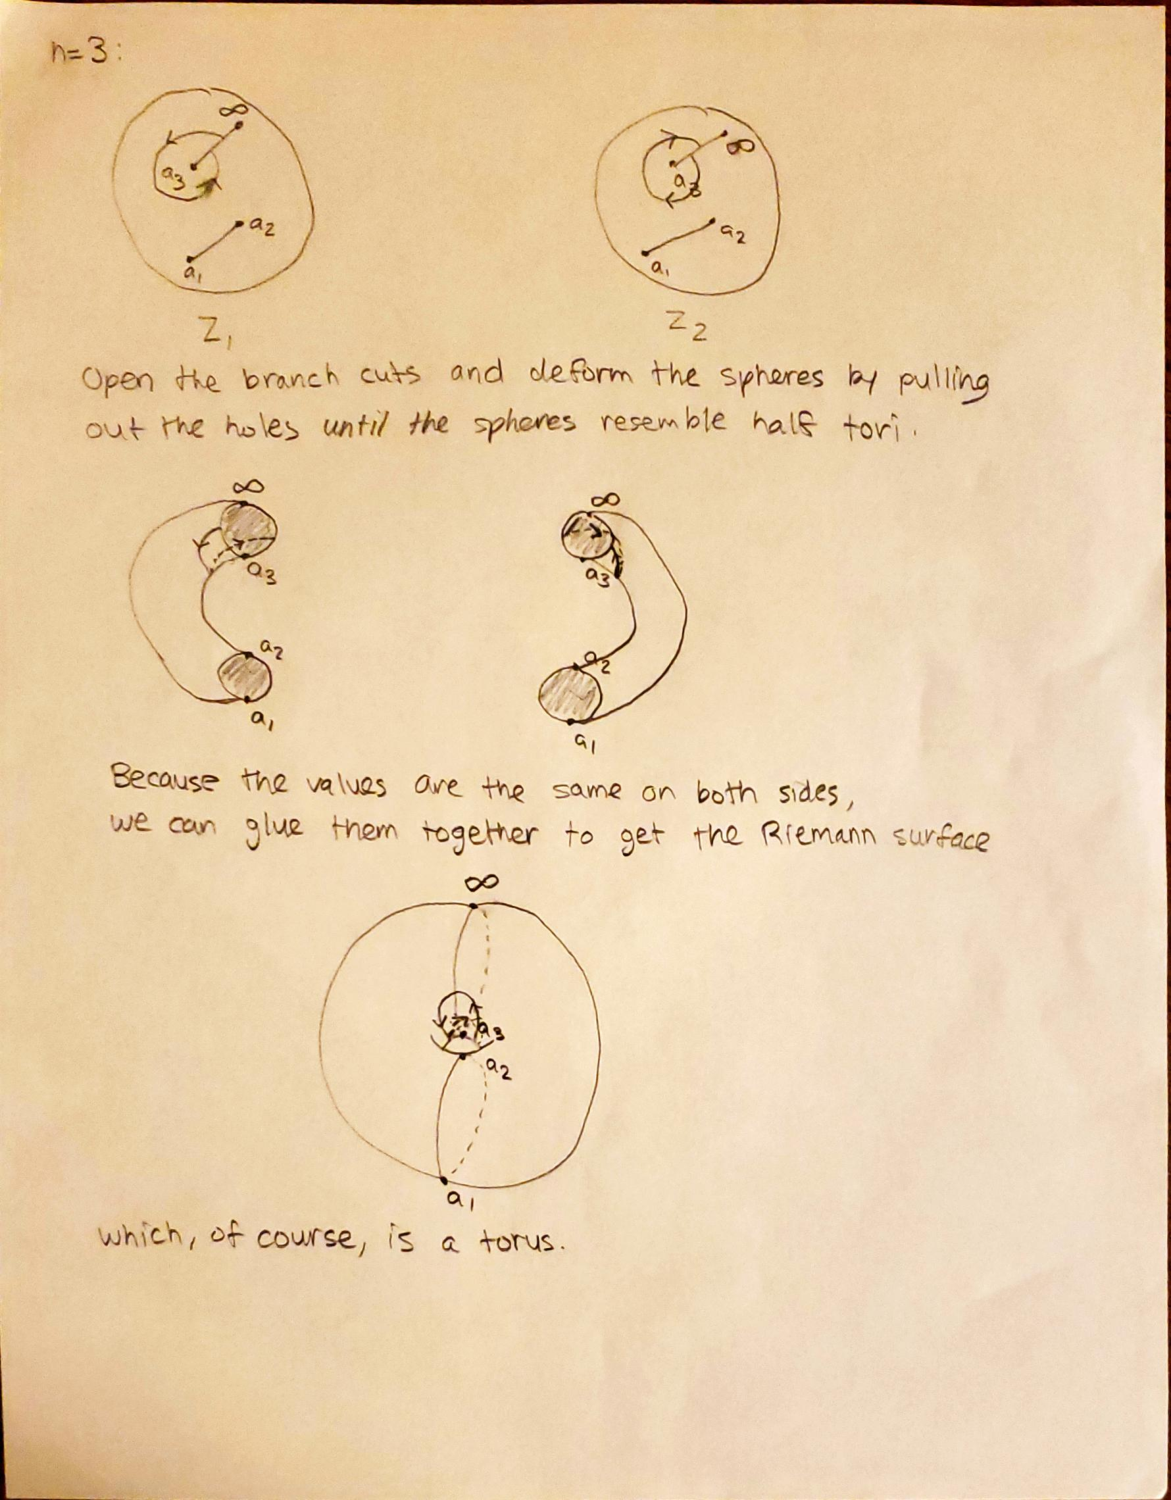
\includegraphics[scale=0.4]{567hw3fig1.pdf}\\
In the case $n=4$, we have the same number of branch points, so everything is the same except $z=a_4$ replaces $\infty$ as a branch point.\\
For the case $n=5$, we have branch points at $a_1, a_2, a_3, a_4, a_5, \infty$, meaning that we can draw 3 branch cuts and do the following:\\
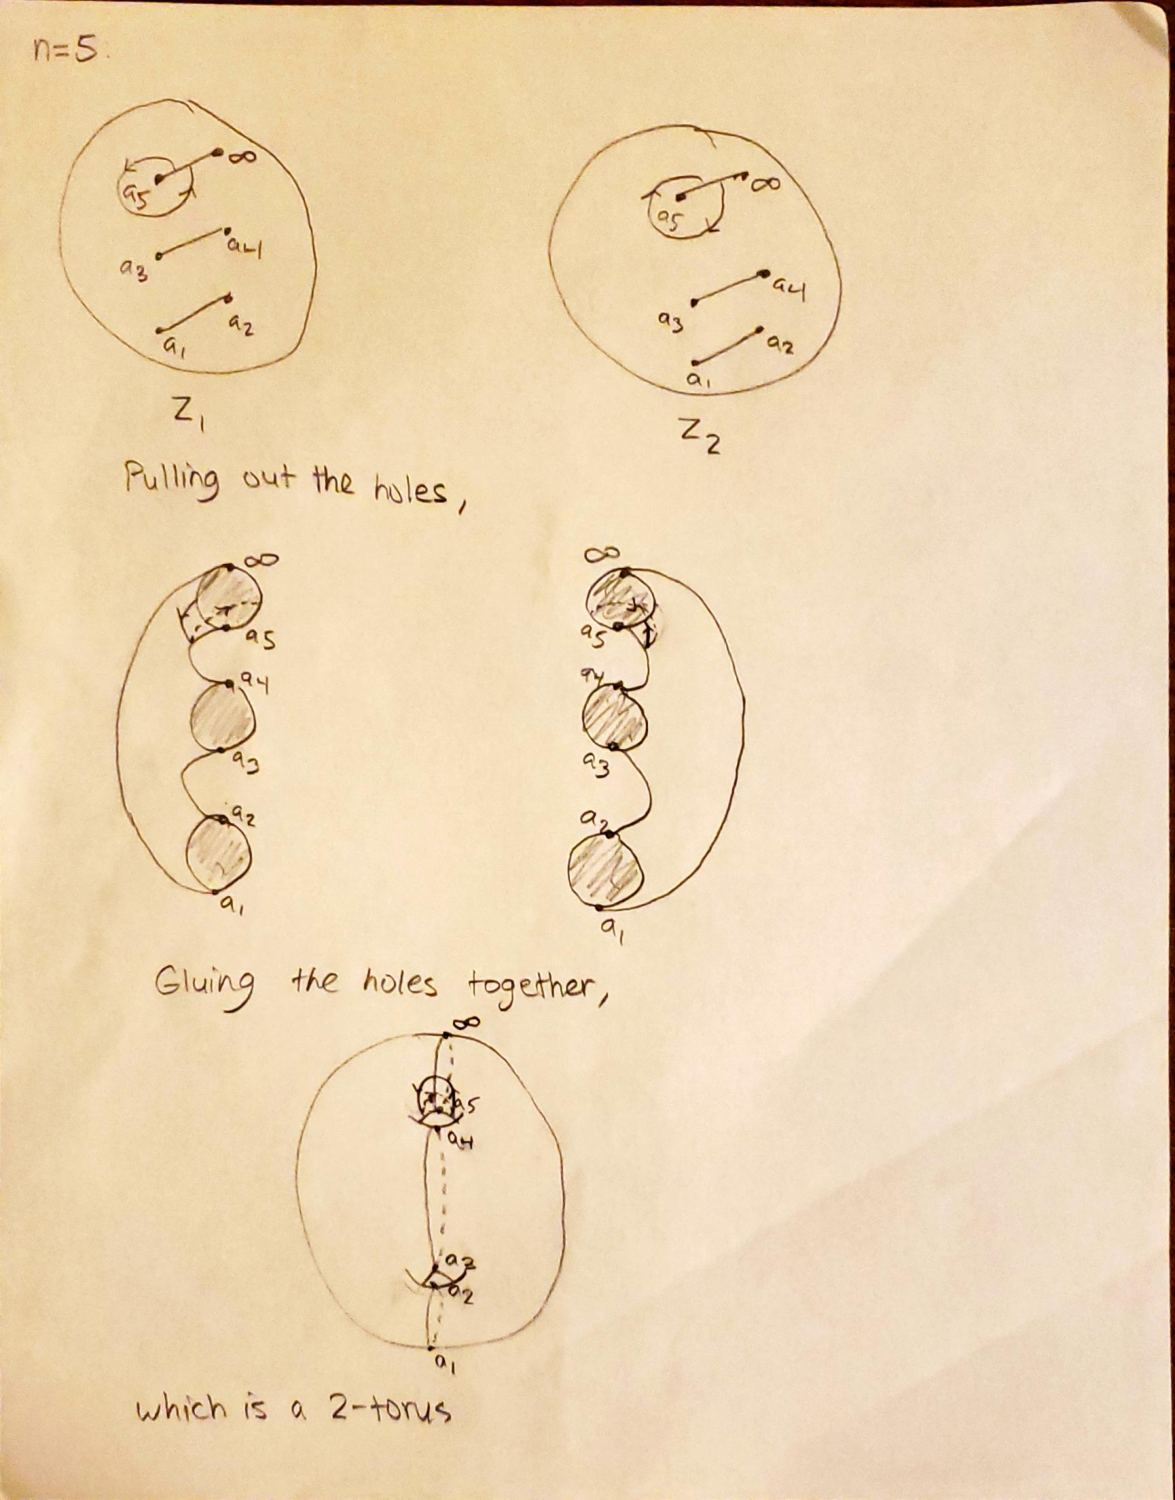
\includegraphics[scale=0.4]{567hw3fig2.pdf}\\
In general, we will have $N$ branch points if $N$ is even and $N+1$ branch points if $N$ is odd, meaning that the Riemann surface will be a k-torus for an even $N=2k$ and an odd $N=2k-1$.

\section{Problem 4 (2.2.7)}
Consider the function $\Omega(z)=k\ln(z-z_0)$ where $k\in\real$ and $z_0\in\mathbb{C}$ are constants. The velocity potential $\phi$ and the stream function $\psi$ are just the real and imaginary parts of this function respectively, so $\Omega(z)=k(\ln|z-z_0|+i\arg(z-z_0))$ gives that $\phi(z)=k\ln|z-z_0|$ and $\psi(z)=k\arg(z-z_0)$.\\
From page 41 of the text, we have that velocity is given by
\[
\overline{\Omega}'(z)=\overline{\frac{k}{z-z_0}}=\frac{k}{\overline{z-z_0}}=\frac{k(z-z_0)}{|z-z_0|^2}.
\]
We wish to show that this is purely radial relative to $z=z_0$, so consider a shifted polar coordinate system such that $z-z_0=Re^{i\theta}$. Then, 
\[
\overline{\Omega}'(z)=\frac{kRe^{i\theta}}{R^2}=\frac{k}{R}e^{i\theta}.
\]
Written in vector form, velocity is $(\frac{k}{R}\cos\theta,\frac{k}{R}\sin\theta)$; this is just a normal vector pointing radially outward from the origin (defined relative to $z_0$) scaled by $\frac{k}{R}$ (as the collection of these vectors is a circle for fixed $R$). Thus, velocity is purely radial relative to $z=z_0$ (given by $V_r=\frac{k}{R}$) .\\
The following are sketches of the flow configuration for different values of k:\\
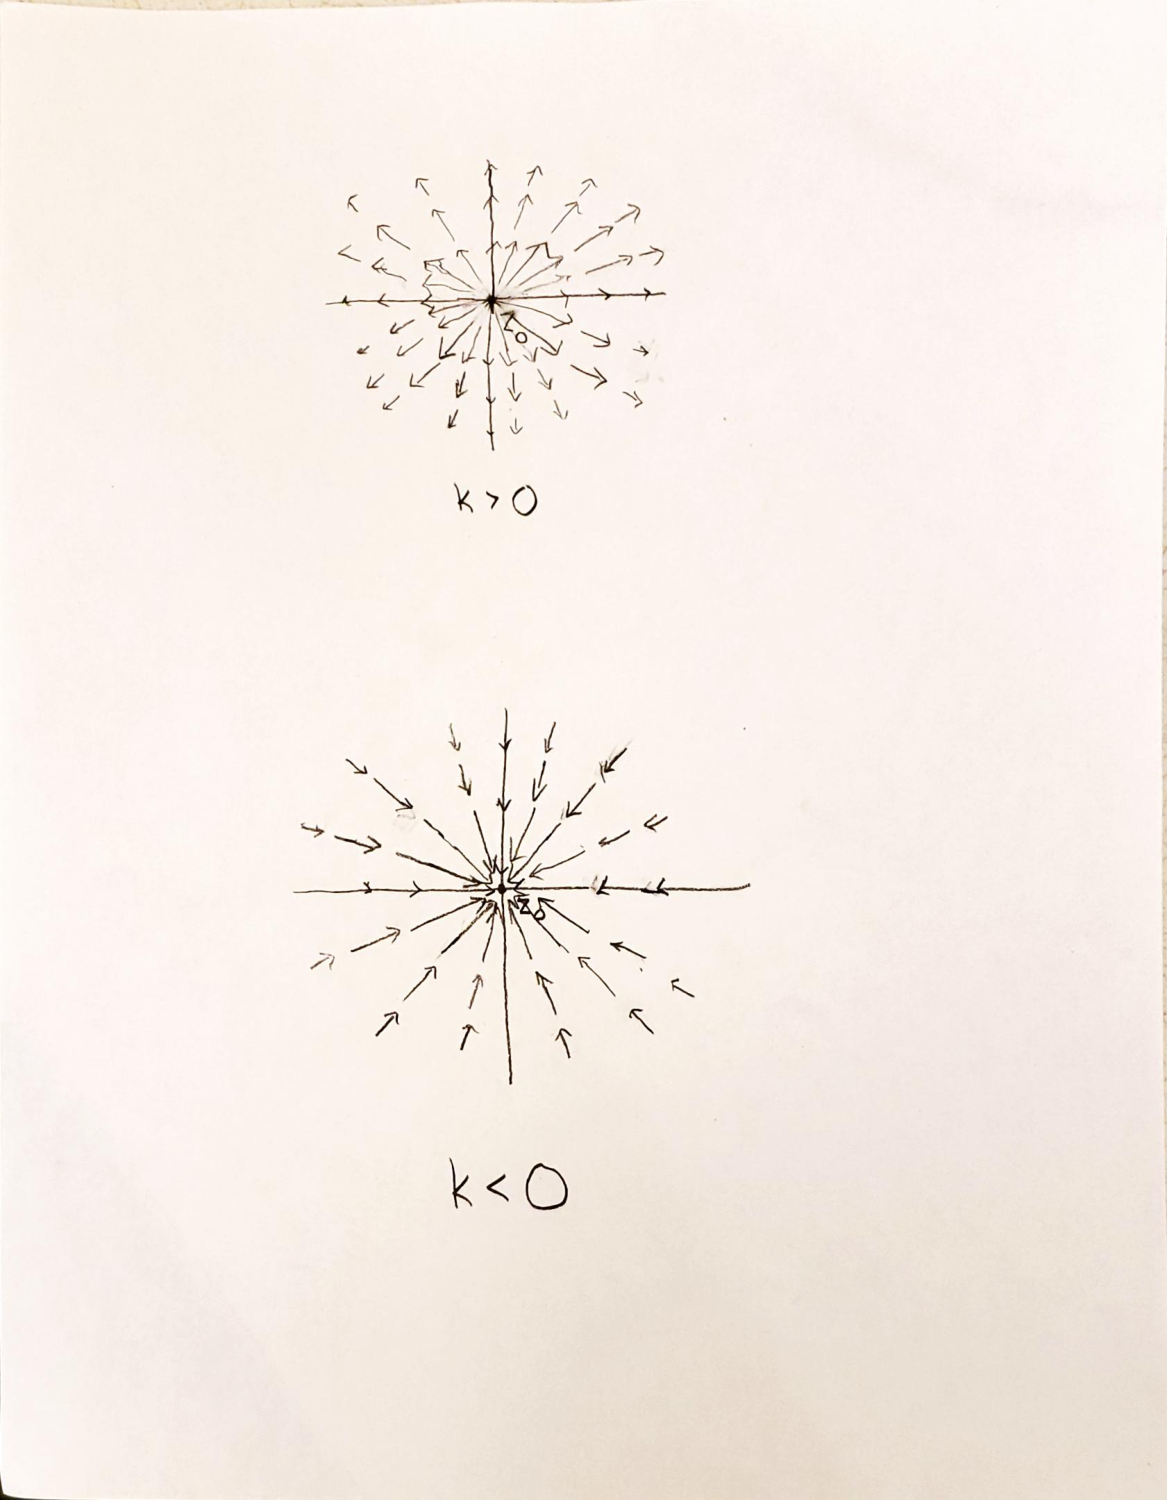
\includegraphics[scale=0.4]{567hw3fig3.pdf}\\
Let $M=\oint_C V_r ds$ where $V_r$ is the radial velocity and $ds$ is the increment of arclength in the direction tangent to the circle $C$ enclosing $z=z_0$. Continuing with our modified coordinate system, let $C=Re^{i\theta}$. Then,
\[
M=\oint_C V_r ds=\int_0^{2\pi}(\frac{k}{R})(Rd\theta)=k\int_0^{2\pi}d\theta=2\pi k.
\]
\end{document}
